\documentclass[10pt]{article}
\usepackage[a4paper,margin=20mm]{geometry}
\usepackage{fontspec}
\setmainfont{Liberation Sans}
\usepackage{amsmath}
\usepackage{graphicx}
\usepackage{booktabs}
\usepackage{caption}
\usepackage{url}
\usepackage{xcolor}
\usepackage[hidelinks]{hyperref}
\captionsetup{font=small,labelfont=bf,justification=justified,singlelinecheck=false}
\setlength{\parskip}{0.4em}
\setlength{\parindent}{0pt}
\definecolor{verdict}{RGB}{170,40,0}

\title{Do task signals use the dimensions of spontaneous activity?\\[0.2em]\large A pilot comparing IBL Neuropixels and mesoscope recordings}
\author{Claude \and International Brain Laboratory (IBL) \and Michael Schartner}
\date{\today}

\begin{document}
\maketitle

\begin{center}
\fcolorbox{verdict}{white}{\parbox{0.94\textwidth}{\color{verdict}\textbf{Verdict: not supported as pre-registered; do not expand the BWM--meso comparison.}\\[0.3em]
\normalsize\color{black} With 30 neurons per region in both modalities, task coding directions are barely more aligned with the top spontaneous dimensions than noise is ($R\approx 0.8$--$1.3$). Motor regions are \emph{not} more aligned than sensory regions, in either modality (pre-registered criteria 1 and 3 fail). In meso, alignment grows strongly with the number of neurons. At $N=200$ motor cortex aligns more than somatosensory cortex for choice in the one animal with both, but this is exploratory, from a single mouse, and confounded with the stimulus. BWM regions are too small to reach that regime.}}
\end{center}

\section{Question and pre-registered hypothesis}

Stringer et al.\ (2019, \emph{Science}) found that in mouse V1, stimulus responses are largely orthogonal to the dominant dimensions of spontaneous, behaviour-related activity. We asked whether this holds for other task variables and outside sensory cortex, using two IBL datasets recorded in the same task: brain-wide-map Neuropixels recordings (BWM; spikes, all depths, subcortex) and mesoscope two-photon imaging (meso; deconvolved calcium, thousands of layer-2/3 neurons in dorsal cortex). Both include a 600-s grey screen (spontaneous activity) in the passive protocol after the task.

The hypothesis, analysis and decision criteria were written to \path{HYPOTHESIS.md} before any analysis (SHA-256 recorded at 15:19 on 23 October 2026):

\begin{quote}
\textbf{H.} The alignment of task coding with spontaneous activity follows the sensory-to-motor hierarchy. In \emph{sensory} regions, task coding directions are not preferentially aligned with the top spontaneous dimensions. In \emph{motor/action} regions, coding directions, especially for choice, lie preferentially in them. The ordering motor~$>$~sensory is the same in both modalities.
\end{quote}

\textbf{Pre-registered criteria for ``promising''.}
\begin{enumerate}
  \item For choice, the median $R$ (defined below) of motor regions exceeds that of sensory regions, in both modalities.
  \item The difference has the same sign in at least 2 of 3 sessions per modality.
  \item The sensory $R$ for stimulus side is $\le 1$ (Stringer et al.\ direction).
\end{enumerate}
If criterion 1 fails in either modality, the hypothesis is not supported and the analysis is not expanded.

\section{Data and methods}

\textbf{Sessions.}
\begin{itemize}
  \item \textbf{BWM:} 5c0c560e (NR\_0028), 6274dda8 (CSH\_ZAD\_025) and 2bdf206a (UCLA037), with good units only (\texttt{label}~$=1$) and Beryl areas. Each session has both region classes with $\ge30$ units.
  \item \textbf{Meso:} 90029e53 (SP054; visual areas, SSp, RSP), fa10ff03 (SP075; MOp/MOs and SSp) and a4afea1e (SP076; MOp/MOs). Allen areas with layers pooled; labels are mostly pre-histology estimates.
\end{itemize}

\textbf{Region classes} (fixed in advance).
\begin{itemize}
  \item \emph{Sensory:} visual (VIS*), auditory and somatosensory cortex; LGd, LP, PO, VPM, VPL, MG; SCs.
  \item \emph{Motor/action:} MOp, MOs; CP, ACB, GPe, SNr; SCm, MRN, PAG; GRN, IRN, PRN; ZI, VAL, VM.
  \item All other regions are reported as \emph{other} and are not tested.
\end{itemize}

\textbf{Spontaneous subspace.} Activity in the grey screen was averaged in 1-s bins (600 bins). Each neuron was z-scored with its grey-screen mean and s.d. PCA was done on the z-scored grey-screen activity; $U_k$ holds the top $k$ PCs ($k=3$ primary, 1--10 as a curve).

\textbf{Task coding directions.} Per-trial window means were computed and z-scored with the same grey-screen statistics. The trial mask required a choice and $0.08\le\mathrm{RT}\le2$~s. The windows follow the dorsal-maps analysis (BWM / meso; meso windows are 0.3~s because of the $\sim$5-Hz frame rate):
\begin{itemize}
  \item \emph{stimulus side}, contrast $\ge 25\%$: stimulus onset $+[0, 0.1]$ / $[0, 0.3]$~s;
  \item \emph{choice}: first movement $+[-0.1, 0]$ / $[-0.3, 0]$~s;
  \item \emph{feedback} (reward vs error): feedback $+[0, 0.2]$ / $[0, 0.3]$~s;
  \item \emph{block prior} ($p_L = 0.8$ vs $0.2$): stimulus onset $+[-0.4, -0.1]$~s.
\end{itemize}
The coding direction is $d$ = mean(class~1) $-$ mean(class~0).

\textbf{Alignment.} $A = \|U_k^\top d\|^2/\|d\|^2$, the fraction of the coding direction that lies in the top-$k$ spontaneous PCs. Isotropic chance is $k/N$.
\begin{itemize}
  \item \emph{Noise null:} we recomputed $A$ for 500 circular shifts of the label sequence (shift $\ge 10\%$ of trials; this keeps class counts and block autocorrelation). This gives the alignment of a coding direction made only of noise with the data's covariance.
  \item \emph{Main statistic:} $R = A/\overline{A_\text{null}}$. $R>1$ means more aligned with spontaneous activity than noise; $R<1$ means more orthogonal.
  \item \emph{Coding:} a region-variable pair counts as coding if $\|d\|^2$ exceeds the 95th percentile of its null (median over draws).
\end{itemize}

\textbf{Matching.} Every region with $\ge 30$ neurons was analysed with $N = 30$ neurons per draw (20 random draws, averaged), so both modalities and all regions have the same dimensionality. All computations ran on the GPU (PyTorch).

\section{Results}

\subsection{Pre-registered test (N = 30)}

\begin{figure}[h]
  \centering
  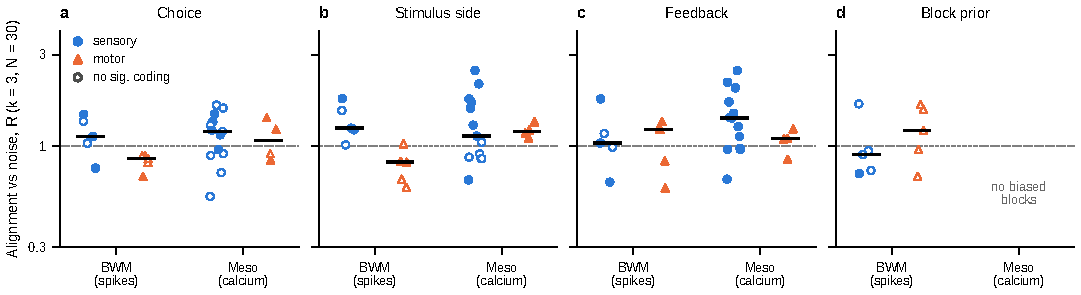
\includegraphics[width=\textwidth]{figures/fig_main.pdf}
  \caption{\textbf{Alignment of task coding with the top 3 spontaneous PCs, relative to noise.} Each marker is one region of one session (20 draws of 30 neurons). Blue circles: sensory regions; orange triangles: motor/action regions. Filled markers: the region codes the variable ($\|d\|^2$ above the 95th percentile of the circular-shift null); open: it does not. Black bars: medians. The dashed line $R=1$ is the alignment of a noise direction. \textbf{a} Choice. \textbf{b} Stimulus side (contrast $\ge 25\%$). \textbf{c} Feedback. \textbf{d} Block prior; the meso sessions have no biased blocks.}
  \label{fig:main}
\end{figure}

\begin{itemize}
  \item \textbf{Alignment is close to the noise level.} Across all region--variable pairs, $R$ ranges from about 0.5 to 2.5, with medians between 0.8 and 1.4 (Fig.~\ref{fig:main}). The coding directions are neither strongly aligned with nor orthogonal to the dominant spontaneous dimensions.
  \item \textbf{Criterion 1 fails in both modalities.} For choice, median $R$ is 0.86 (motor) vs 1.13 (sensory) in BWM, and 1.07 vs 1.20 in meso. The ordering is the opposite of the hypothesis.
  \item \textbf{Criterion 2.} In BWM, sensory exceeds motor for choice in 2 of 3 sessions (5c0c560e: 1.41 vs 0.80; 2bdf206a: 1.08 vs 0.82; 6274dda8: 0.77 vs 0.88). In meso only SP075 has both classes, where motor is marginally higher (1.32 vs 1.25). So the criterion cannot be assessed properly in meso.
  \item \textbf{Criterion 3 fails.} Sensory $R$ for stimulus side is 1.24 (BWM) and 1.13 (meso): slightly \emph{more} aligned than noise, not orthogonal as in Stringer et al. The meso stimulus window overlaps movement, however (see Limitations).
  \item \textbf{The ordering does not depend on $k$.} With $k$ from 1 to 10, BWM motor regions stay below sensory regions for choice, and in meso the two classes converge towards 1 (Fig.~\ref{fig:k}a,b).
\end{itemize}

\begin{figure}[h]
  \centering
  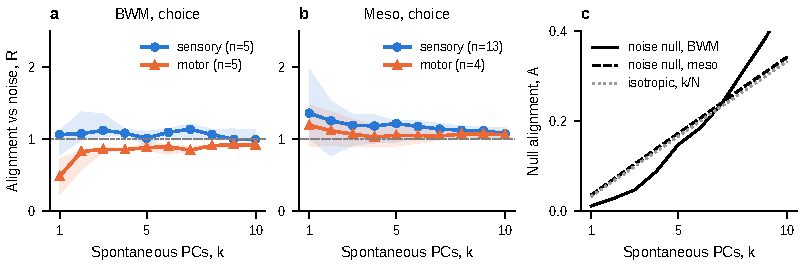
\includegraphics[width=0.75\textwidth]{figures/fig_k.pdf}
  \caption{\textbf{Dependence on the number of spontaneous PCs.} \textbf{a} BWM, choice: median $R$ (lines) and interquartile range (bands) per class as a function of $k$. \textbf{b} The same for meso. \textbf{c} Median null alignment $A_\text{null}$ against isotropic chance $k/N$. Meso noise is close to isotropic. BWM noise lies \emph{less} in the top spontaneous PCs than isotropic noise for $k<7$: Poisson noise in short task windows dominates, and low-rate units with large z-scores contribute little to the top grey-screen PCs.}
  \label{fig:k}
\end{figure}

\subsection{Sensitivity analyses (added in review, not pre-registered)}

\begin{table}[h]
\centering\small
\caption{\textbf{Median $R$ for choice ($k=3$) under alternative choices.} Values in brackets use only regions that significantly code choice.}
\label{tab:sens}
\begin{tabular}{lcc}
\toprule
Analysis & Motor & Sensory \\
\midrule
Pre-registered, BWM ($N=30$, 1-s grey bins) & 0.86 (0.80) & 1.13 (1.13) \\
BWM, 0.1-s grey bins & 0.81 (0.94) & 1.18 (1.10) \\
BWM, units $\ge 1$~Hz in the grey screen & 0.60 (0.49) & 1.16 (1.29) \\
Pre-registered, meso ($N=30$) & 1.07 (1.23) & 1.20 (1.21) \\
Meso, $N=200$ (regions with $\ge 200$ neurons) & 2.46 (2.46) & 1.46 (1.84) \\
\bottomrule
\end{tabular}
\end{table}

\begin{itemize}
  \item \textbf{BWM:} the motor $<$ sensory ordering survives 0.1-s grey-screen bins and the exclusion of low-rate units (Table~\ref{tab:sens}).
  \item \textbf{Meso depends on the number of neurons.} With more neurons per draw, noise directions spread over more dimensions ($A_\text{null}$ falls as $k/N$), while coding directions keep their part in the shared spontaneous subspace, so $R$ grows (Fig.~\ref{fig:nsweep}a--c). At $N=30$ motor and sensory regions are indistinguishable for choice (1.19 vs 1.13, regions with $\ge 200$ neurons). At $N=200$ motor is clearly higher (2.98 vs 1.51). The same holds for stimulus side (3.70 vs 2.23), but not for feedback (3.18 vs 2.85).
  \item \textbf{SP075, the only meso animal with both classes:} at $N=200$, choice coding is more aligned in MOp and MOs ($R=4.1$, 3.4) than in any somatosensory area (0.7--2.1). Somatosensory areas are as aligned as motor areas for stimulus side and feedback (Fig.~\ref{fig:nsweep}d). This choice-specific pattern is in line with the hypothesis, but it comes from one mouse and was not pre-registered.
\end{itemize}

\begin{figure}[h]
  \centering
  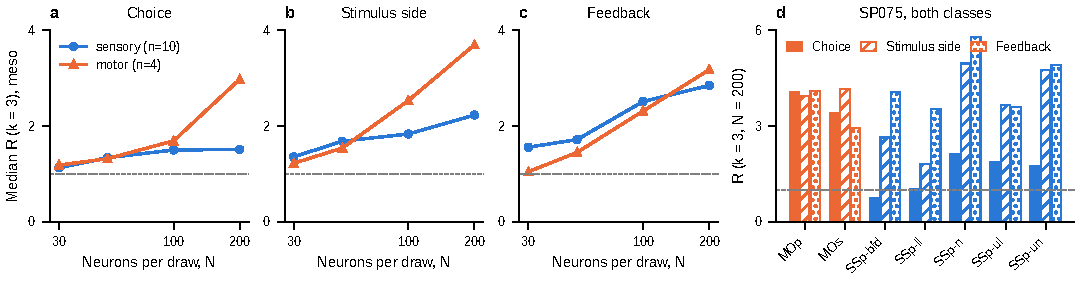
\includegraphics[width=\textwidth]{figures/fig_nsweep.pdf}
  \caption{\textbf{Meso alignment depends on the number of neurons (exploratory).} \textbf{a--c} Median $R$ ($k=3$) against neurons per draw $N$ for choice, stimulus side and feedback, in meso regions with $\ge 200$ neurons (10 sensory, 4 motor region-sessions), so the same regions enter at every $N$. \textbf{d} SP075 (fa10ff03) at $N=200$: $R$ per region for choice (filled), stimulus side (hatched) and feedback (dotted). Orange: motor cortex; blue: somatosensory cortex.}
  \label{fig:nsweep}
\end{figure}

\section{Reviews}

\textbf{Round 1 (self-review).}
\begin{itemize}
  \item \emph{Synthetic test:} a coding direction planted inside the top spontaneous PCs gave $R>1$; an orthogonal one gave $R\to 0$; pure noise gave $R\approx 1$ with a wide spread (0.2--1.2 across repeats). The metric works, but $R$ is noisy unless coding is strong.
  \item \emph{Ceiling:} $R$ cannot exceed $1/A_\text{null}$. This is not binding in the data ($A_\text{null}\approx 0.04$--$0.11$, similar for both classes).
  \item \emph{Sensitivity analyses and neuron-count sweep:} Table~\ref{tab:sens}, Fig.~\ref{fig:nsweep}.
\end{itemize}

\textbf{Round 2 (independent agent review, no access to these conclusions).}
\begin{itemize}
  \item \emph{Re-implementation:} a float64 version with eigendecomposition and explicit class means and shifts reproduced 8 values of $A$, $A_\text{null}$ and $R$ to 4 decimals. No code bugs that change the numbers were found. Sign conventions, PCA orientation, null construction and meso interpolation were checked.
  \item \emph{Deviations from the plan,} all reported here: the meso prior is untestable; extra trial rules (at least 20 trials per class, frame gaps, no overlap with the grey screen); zero-variance units dropped; the coding criterion is the median over draws of per-draw percentiles.
  \item \emph{Main inferential concerns,} adopted below: the dependence of $R$ on $N$; different noise floors in the two modalities; shrinkage of $R$ towards 1 when coding is weak; and the stimulus--choice confound.
\end{itemize}

\section{Limitations}
\begin{itemize}
  \item \textbf{Stimulus and choice are confounded.} On trials with $\ge 25\%$ contrast, the stimulus side matches the choice on 95--99\% (BWM) and 72--91\% (meso) of trials. With median RT 0.14--0.18~s, the choice window ends shortly after the stimulus window, and in meso the two overlap on almost every trial. The choice direction is therefore largely the stimulus direction.
  \item \textbf{The regions differ between modalities.} BWM motor regions are all midbrain (MRN, SCm, PAG), while meso motor regions are MOp and MOs only. Only one meso animal has both classes.
  \item \textbf{$R$ depends on $N$, and BWM cannot follow meso.} BWM regions have 32--84 units, so the larger-$N$ regime in which meso shows structure cannot be reached in BWM. In small BWM regions the 20 draws are nearly identical.
  \item \textbf{The noise floors differ.} BWM noise is less aligned with the top spontaneous PCs than isotropic noise (Fig.~\ref{fig:k}c), so $R$ mixes geometry with the noise scaling of each modality.
  \item \textbf{No multiple-comparison control} in the coding criterion ($\sim$100 pairs). Three sessions per modality is descriptive only.
  \item \textbf{Timing:} meso window values use frame times of the first ROI and ignore sub-frame scan offsets.
\end{itemize}

\section{Conclusions}
\begin{enumerate}
  \item \textbf{The pre-registered hypothesis is not supported.} At matched $N=30$, motor regions are not more aligned with spontaneous activity than sensory regions, in either modality. The BWM ordering is, if anything, reversed and robust to the analysis choices tested.
  \item \textbf{The cross-modal comparison is not a good use of this metric.} Alignment relative to noise depends on population size and on the noise model, and BWM regions are too small to reach the regime where meso shows structure. Expanding to more BWM sessions would not change that.
  \item \textbf{Meso is the only route worth considering.} At $N\ge 100$, meso alignment is well above noise, and in SP075 choice coding is more aligned in motor than in somatosensory cortex. Before any expansion, this needs (i) a new pre-registration at a fixed large $N$; (ii) sessions with motor and sensory cortex in the same animal (e.g.\ SP081 c29d0d5a and 19ac39ab, which have 600-s grey screens); and (iii) choice decorrelated from the stimulus (0\% contrast trials, or windows after stimulus encoding).
\end{enumerate}

\textbf{Code and data.} \path{mesoscope/pilot_analyses/meso_ephys_alignment}: \path{HYPOTHESIS.md} (+ hash), \path{extract.py}, \path{analyze.py}, \path{sensitivity.py}, \path{figures.py}; outputs in \path{output/}.

\end{document}
